\chapter{Phase 2: System Interaktion und Bedienung}

\section{User Stories}

Nun werden die Usecases aus Phase 1 mithilfe von User Stories weiter beschrieben. Dabei liegt der Fokus auf Szenarien, die eine Interaktion mit dem Smartwatch-System abbilden.
Die ersten beiden User Stories beschreiben zunächst einen typischen Hauptanwendungsfall der Uhr: Das Annehmen/Ablehnen/Tätigen von Anrufen von dem verbundenen Smartphone.
Um dem Produkt eine detailgetreue Anleitung für einen reibungslosen Einrichtungsprozess beizulegen, wurde eine User Story speziell für das Einrichten, bzw. Koppeln der Smartwatch mit einem Smartphone definiert.
Da eine Kernfunktionion der Smartwatch darin besteht, sie für Fitness-Tracking verschiedener sportlichen Aktivitäten einzusetzen, wurden mehrere User Stories für diese Anwendungsfälle entworfen. Im folgenden wird die User Story "Joggen gehen" beschrieben, weitere Fitness-User Stories finden sich im Anhang an diese Arbeit.
\begin{figure}[H]
\centering\
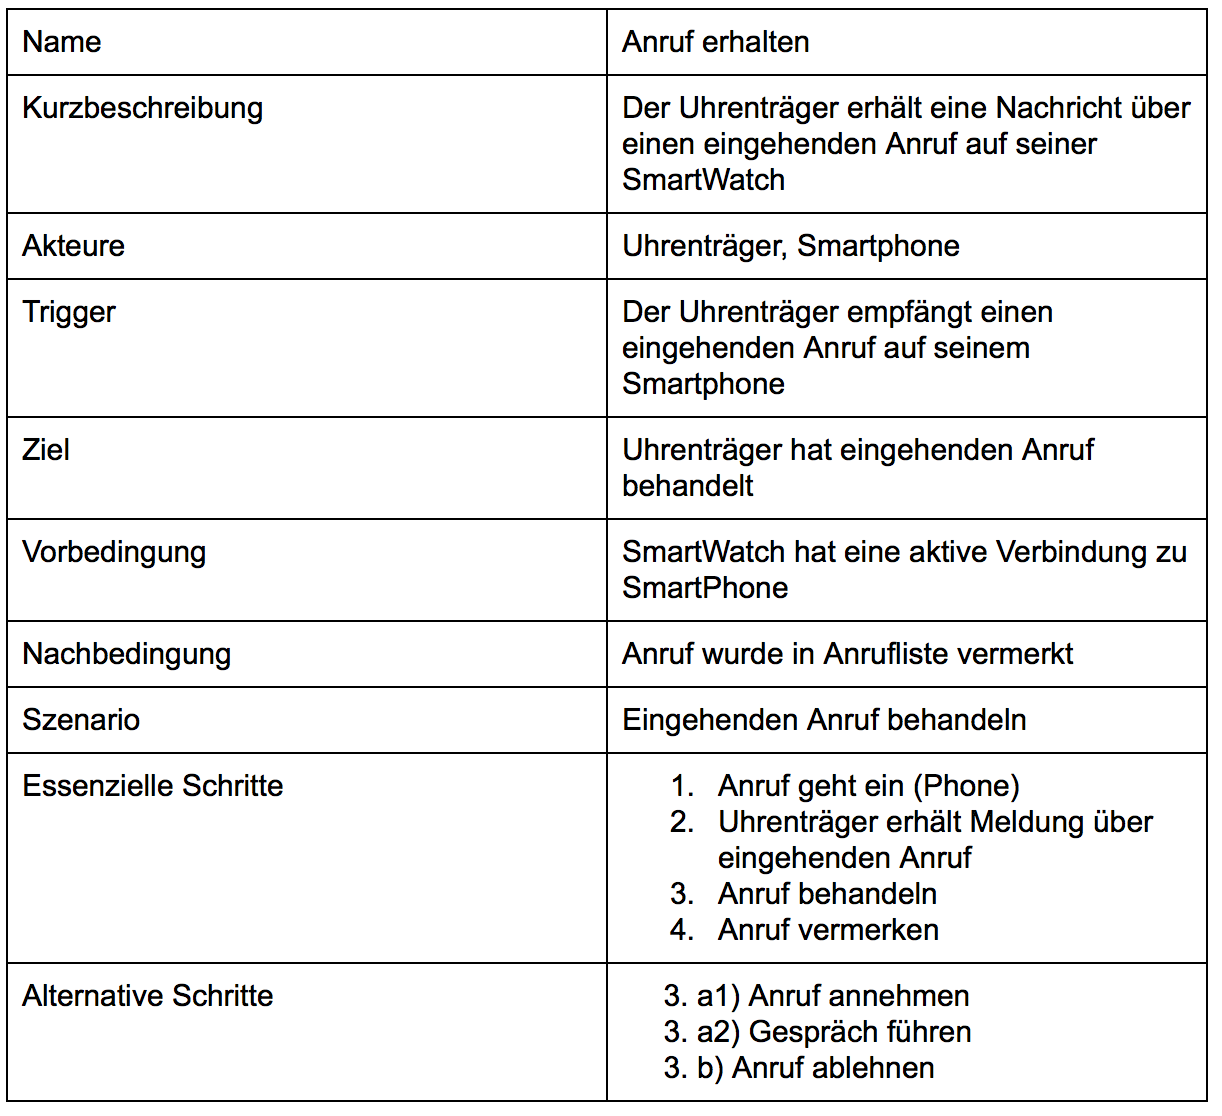
\includegraphics[width=10cm]{img/story_in}
\caption{User Story - Eingehender Anruf}\label{fig:story-in}
\end{figure}
\begin{figure}[H]
\centering\
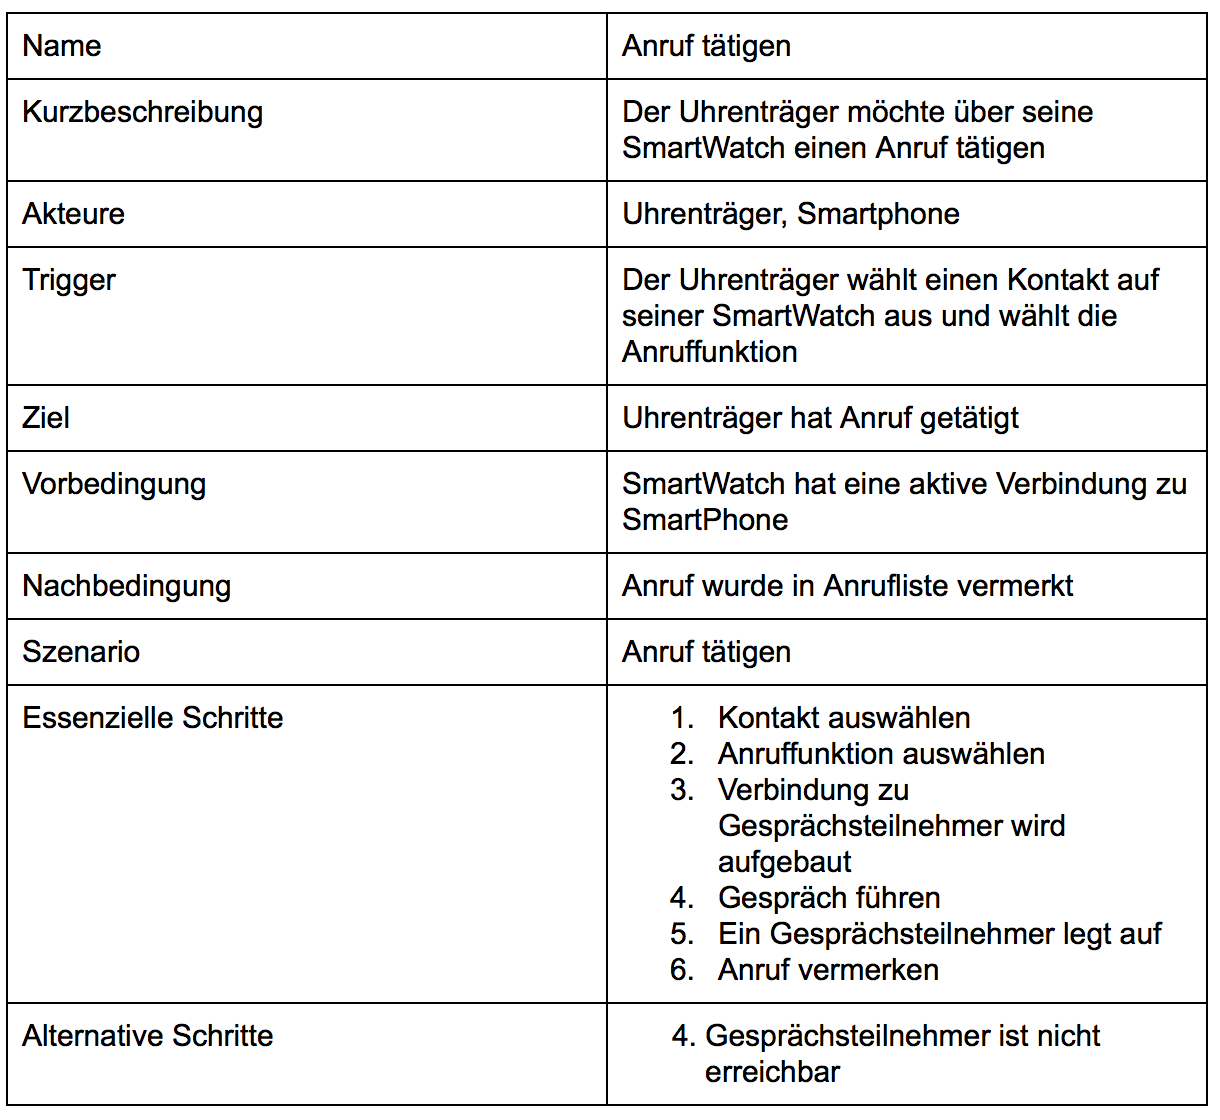
\includegraphics[width=10cm]{img/story_out}
\caption{User Story - Anruf tätigen}\label{fig:story-out}
\end{figure}
\begin{figure}[H]
\centering\
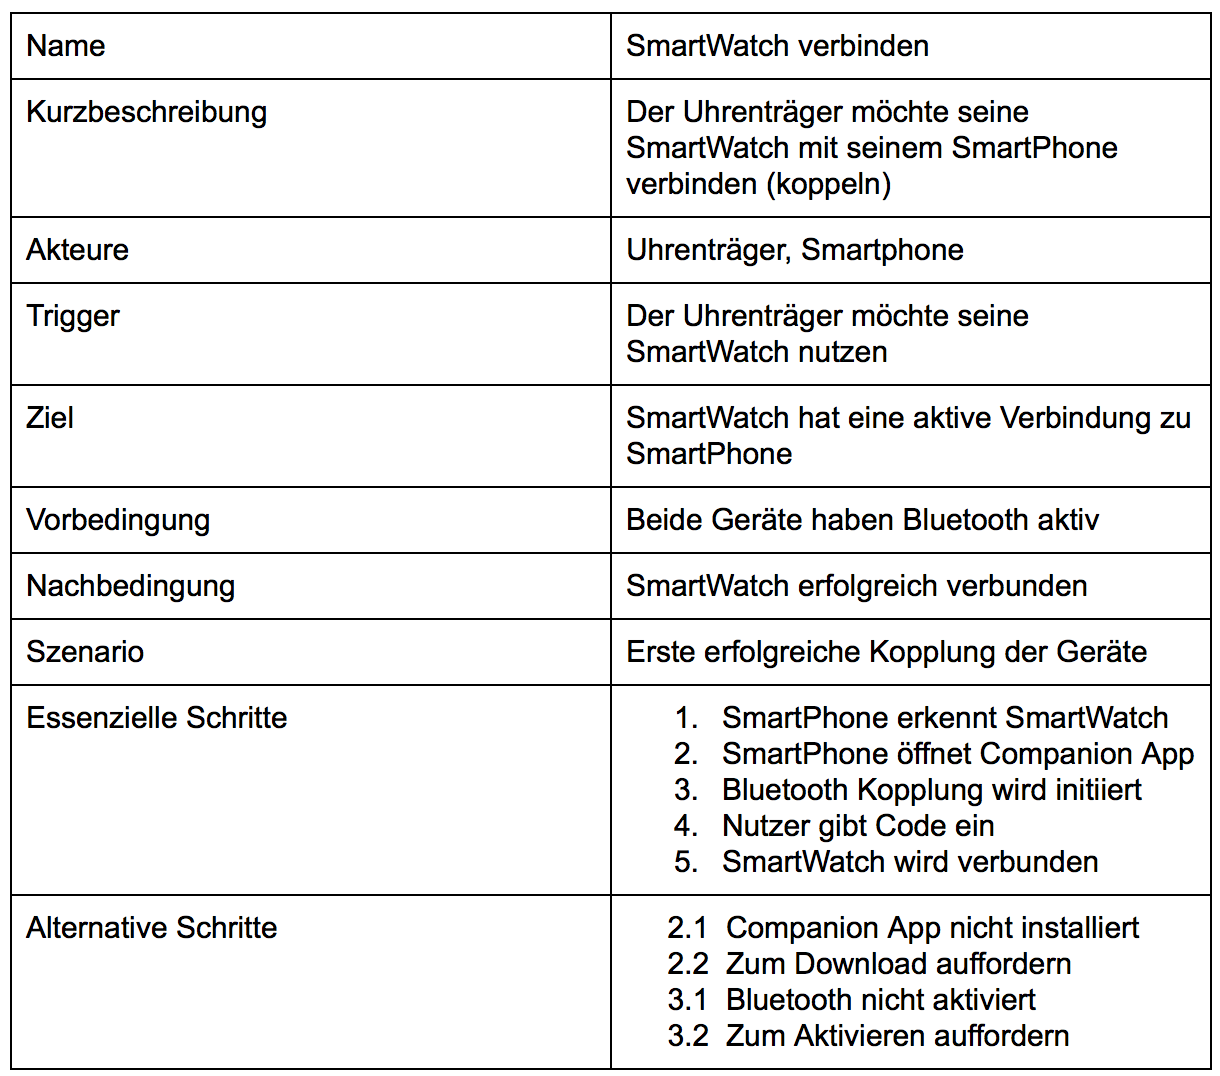
\includegraphics[width=10cm]{img/story_pairing}
\caption{User Story - Pairing}\label{fig:story-pairing}
\end{figure}
\begin{figure}[H]
\centering\
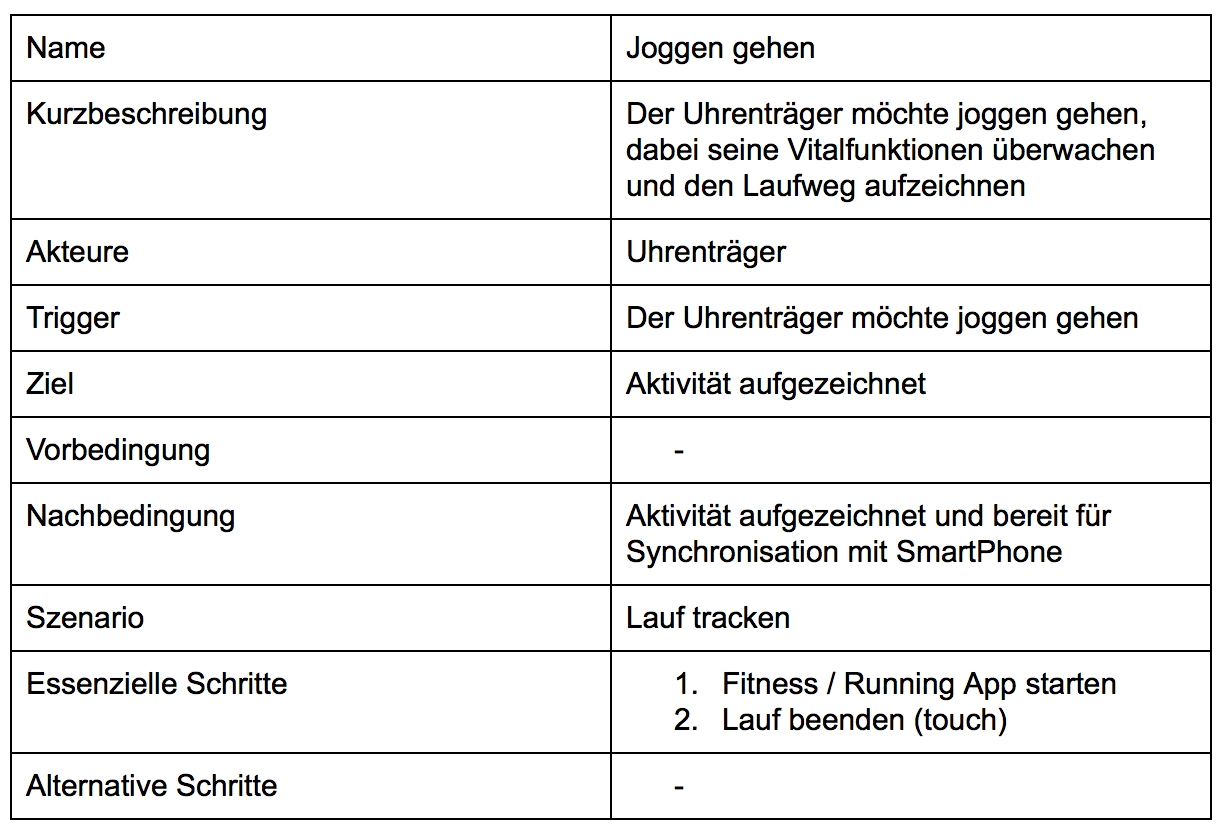
\includegraphics[width=10cm]{img/story_joggen}
\caption{User Story - Fitness}\label{fig:story-joggen}
\end{figure}

\section{Sequence Diagram}
Das Interaktionsverhalten für die Szenarien ``Anruf'' und ``Koppeln'' des Smartwatches mit dem Smartphone, ist fest definiert. Sequenzdiagramme eignen sich hier zur Kontextabgrenzung sehr gut.
In der Abbildung \ref{fig:kopplung} ist der Bluetooth-Kopplungsvorgang als Sequnzdiagramm abgebildet.
Zuerst startet das Smartphone über Bluetooth eine Discovery-Anfrage in der Umgebung.
Das Bluetooth des Smartphones sucht alle verfügbaren Bluetooth-Geräte in der Nähe und übergibt diese dem Smartphone für die Anzeige.
Der Benutzer kann seinen Smartwatch in der Liste auswählen um die Kopplung zu starten.
Danach wird der Benutzer aufgefordert auf seinem Smartphone jetzt die Bluetooth-Kopplungsanforderung mit dem Kopplungs-Code zu bestätigen. Der Kopplungs-Code wird in der Smartwatch angezeigt.
Falls der Benutzer einen falschen Code eingegeben hat, wird die Kopplung vom Smartwatch
abgelehnt.

\begin{figure}[H]
\centering\
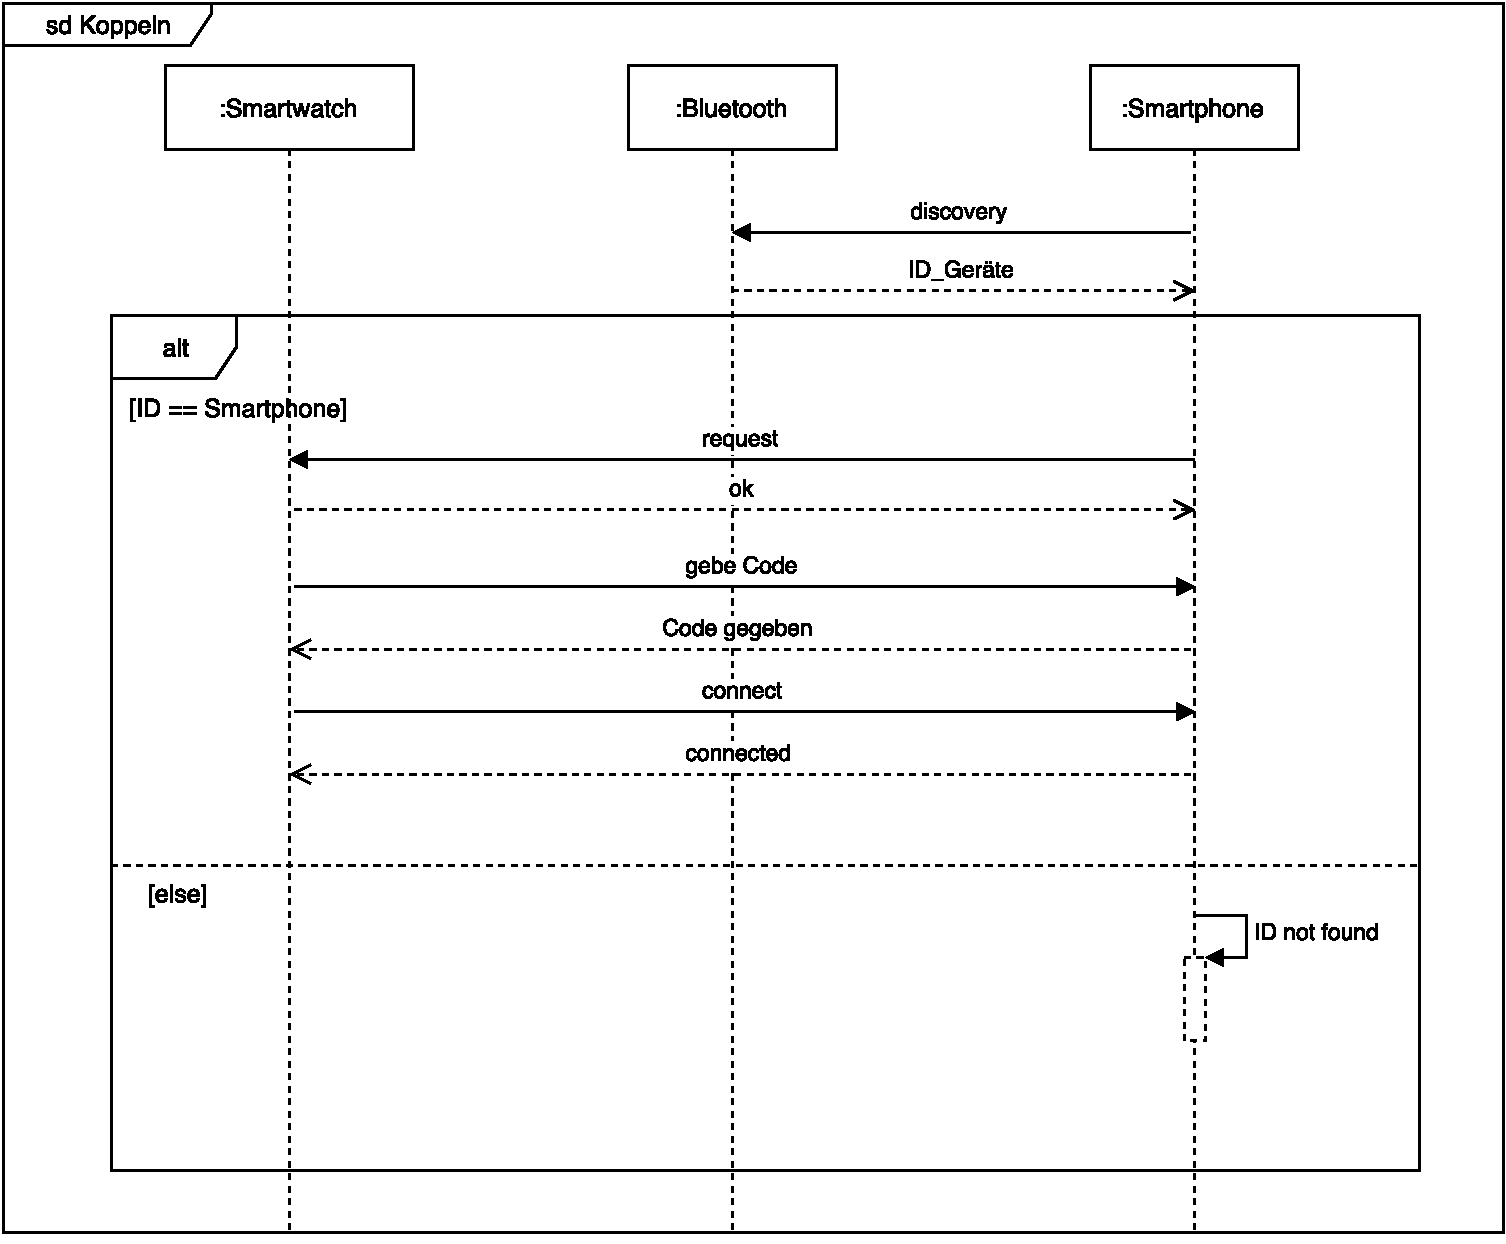
\includegraphics[width=10cm]{img/KoppelnSequenz}
\caption{Kopplung des Smartphones mit Smartwatch}\label{fig:kopplung}
\end{figure}


\begin{figure}[H]
\centering\
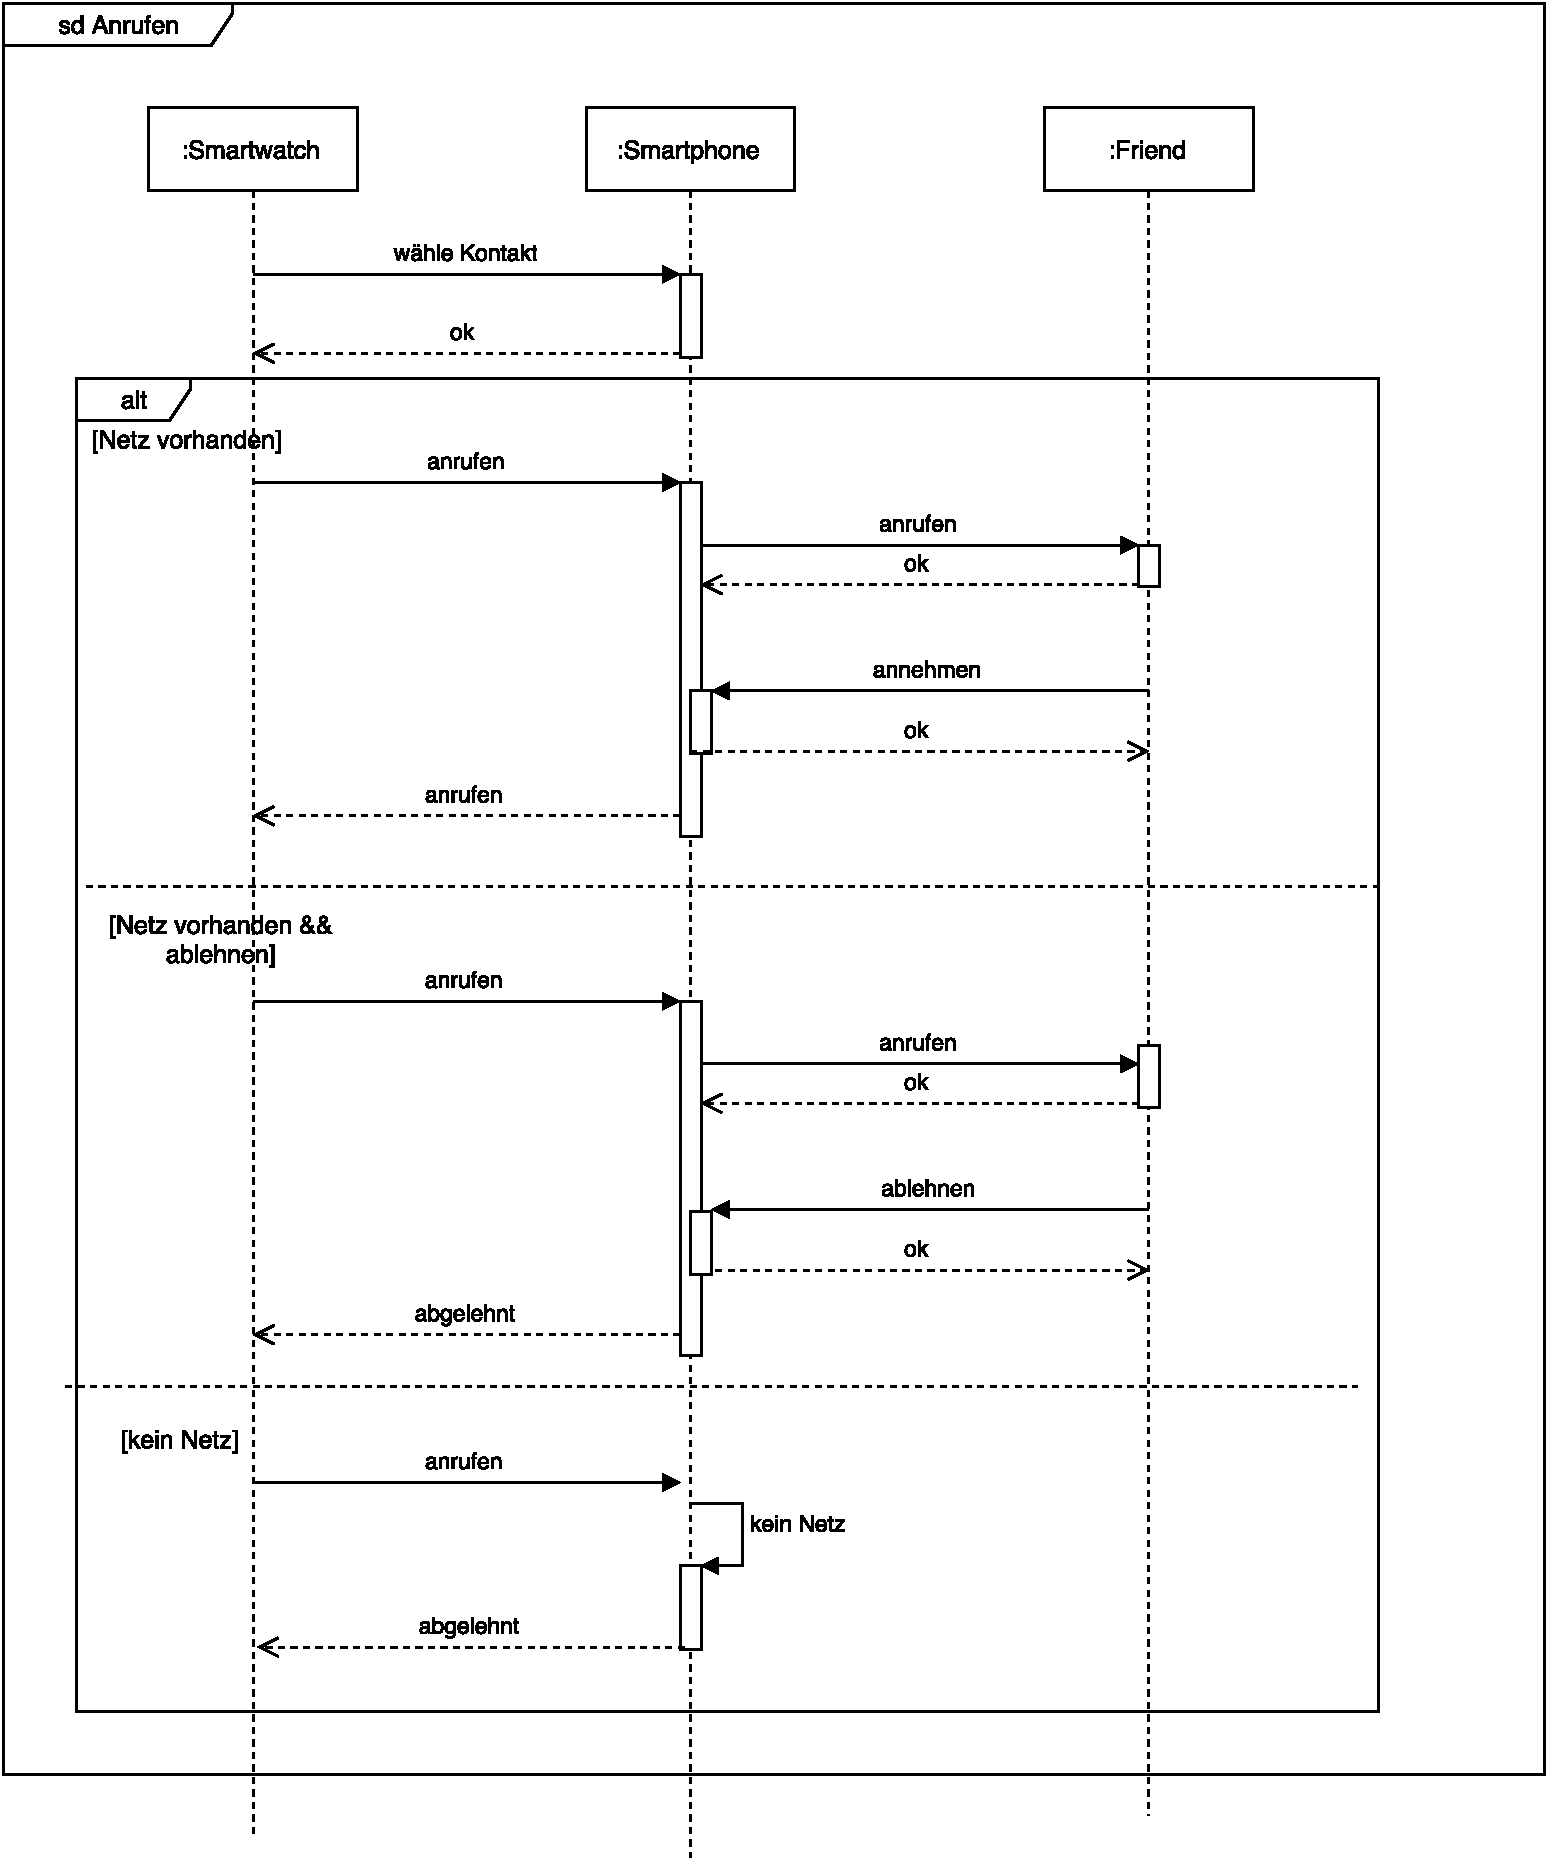
\includegraphics[width=10cm]{img/AnrufenSequenz}
\caption{Anfrufen mit dem Smartwatch}\label{fig:anruf}
\end{figure}



\section{State Diagrams}
Die \textbf{State Diagram} in \textbf{Phase 2} werden dazu benutzt, um das interne Verhalten der \textit{SmartWatch} bei ausgewählten Benutzerinteraktionen darzustellen. Die Diagramme definieren, das Verhalten und die Bearbeitung bei einzelnen Eingaben. Zu diesem Zeitpunkt der Entwicklungsphase wurden die Zustände für die \textit{Verbindung zum Smartphone} \textit{(Pairing)}, das Verwenden der \textit{Fitnessapplikationen} und deren \textit{Speicherfunktion}, sowie das Verhalten bei \textit{ein- und ausgehenden Anrufen} modelliert.\\
\begin{figure}[h]
\centering\
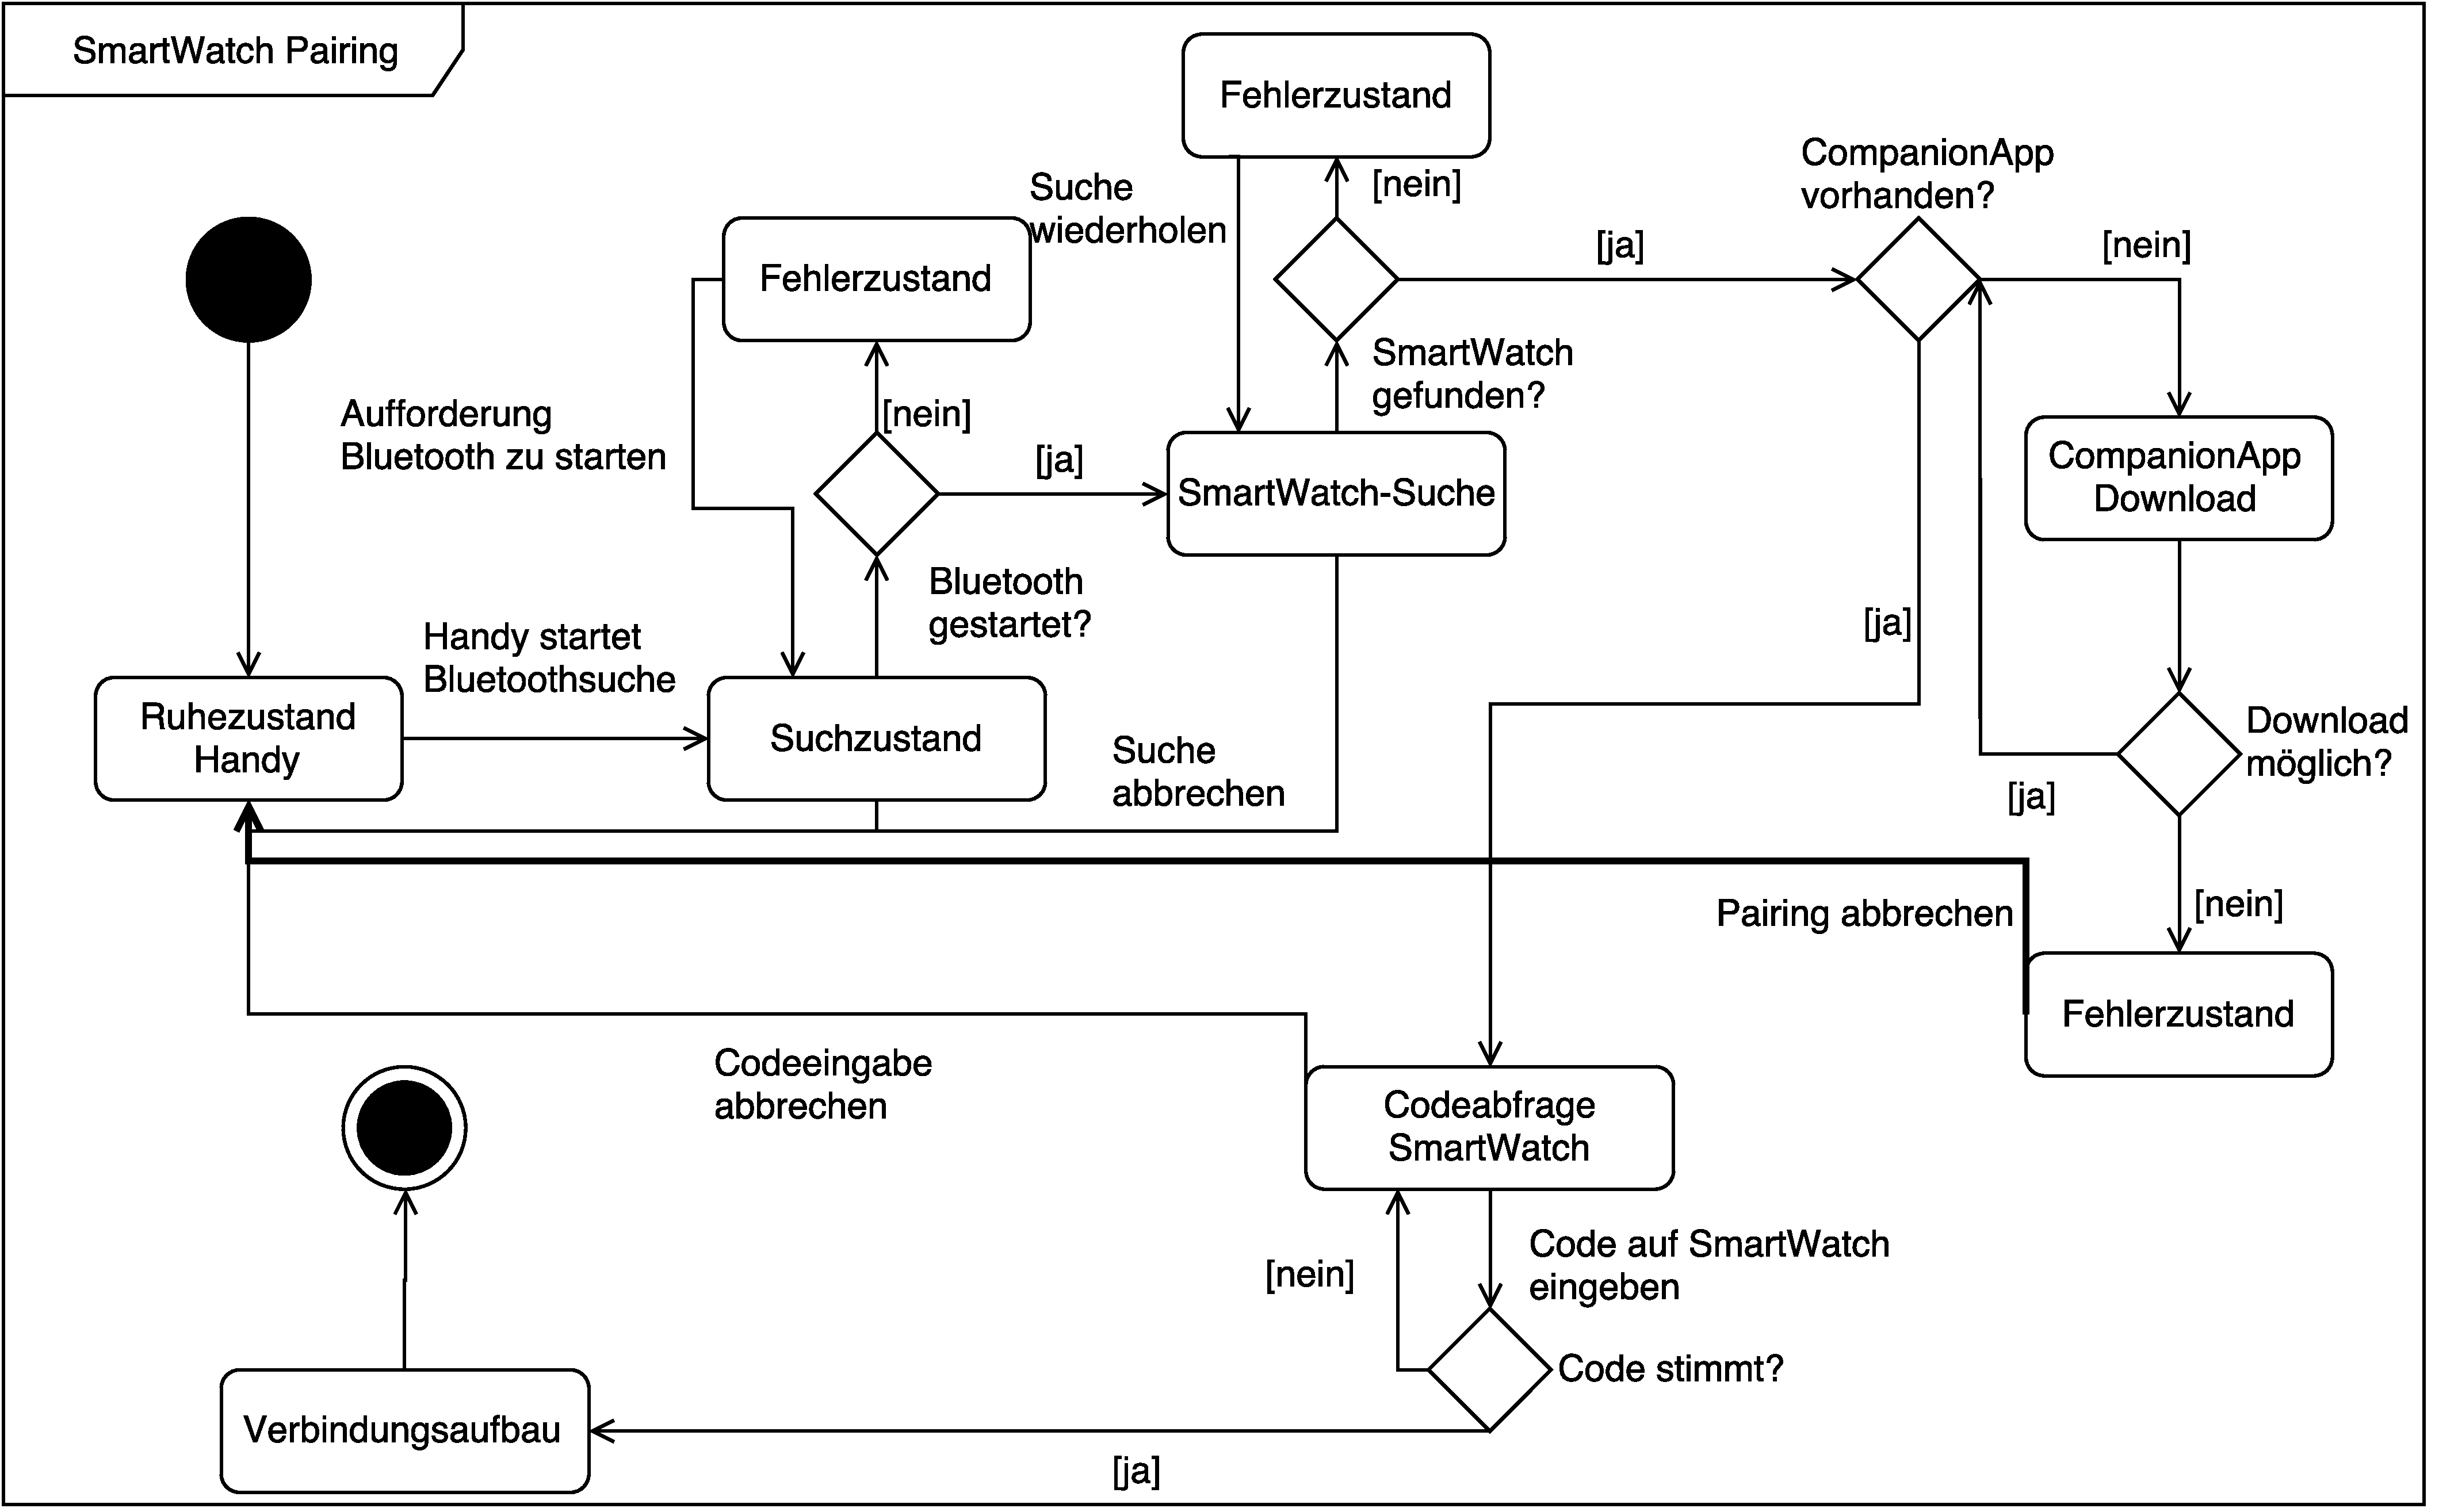
\includegraphics[width=\textwidth]{img/statePairing}
\caption[State Diagram: Pairing]{Verhalten der SmartWatch beim Pairing mit dem SmartPhone.}
\label{fig:statePairing}
\end{figure}
Wenn sich die \textit{SmartWatch} mit dem \textit{SmartPhone} verbinden will, wird zunächst beim Handy mittels \textit{Bluetooth} nach der \textit{SmartWatch} gesucht. Dabei muss bei \textbf{beiden} Geräten das \textit{Bluetooth-Modul} aktiviert sein, da sonst keine Verbindung möglich ist. Wenn sich die Geräte gegenseitig gefunden haben, wird überprüft ob sich auf dem \textit{SmartPhone} die zur \textit{SmartWatch} dazugehörige \textit{Companion-App} befindet. Sollte diese noch nicht installiert sein, wird der Benutzer dazu aufgefordert dies zu tun. Ohne die installierte \textit{Companion-App} ist ein \textit{Pairing} nicht möglich. Wenn die App funktionstüchtig ist, wird Benutzer aufgefordert den vom \textit{SmartPhone} generierten Code auf der \textit{SmartWatch} einzugeben.Dies dient dazu, dass nicht willkürliche \textit{SmartPhones} sich mit der \textit{SmartWatch} verbinden können. Wenn der Code erfolgreich eingegeben wurde, erfolgt die Verbindung zwischen beiden Geräten. Bei jedem der Schritte zum Verbindungsaufbau ist es möglich, den Vorgang abzubrechen und \textit{SmartPhone} und \textit{SmartWatch} in den Ruhenzustand zurück zu versetzen Abb. \ref{fig:statePairing}.\\
\begin{figure}[h]
\centering\
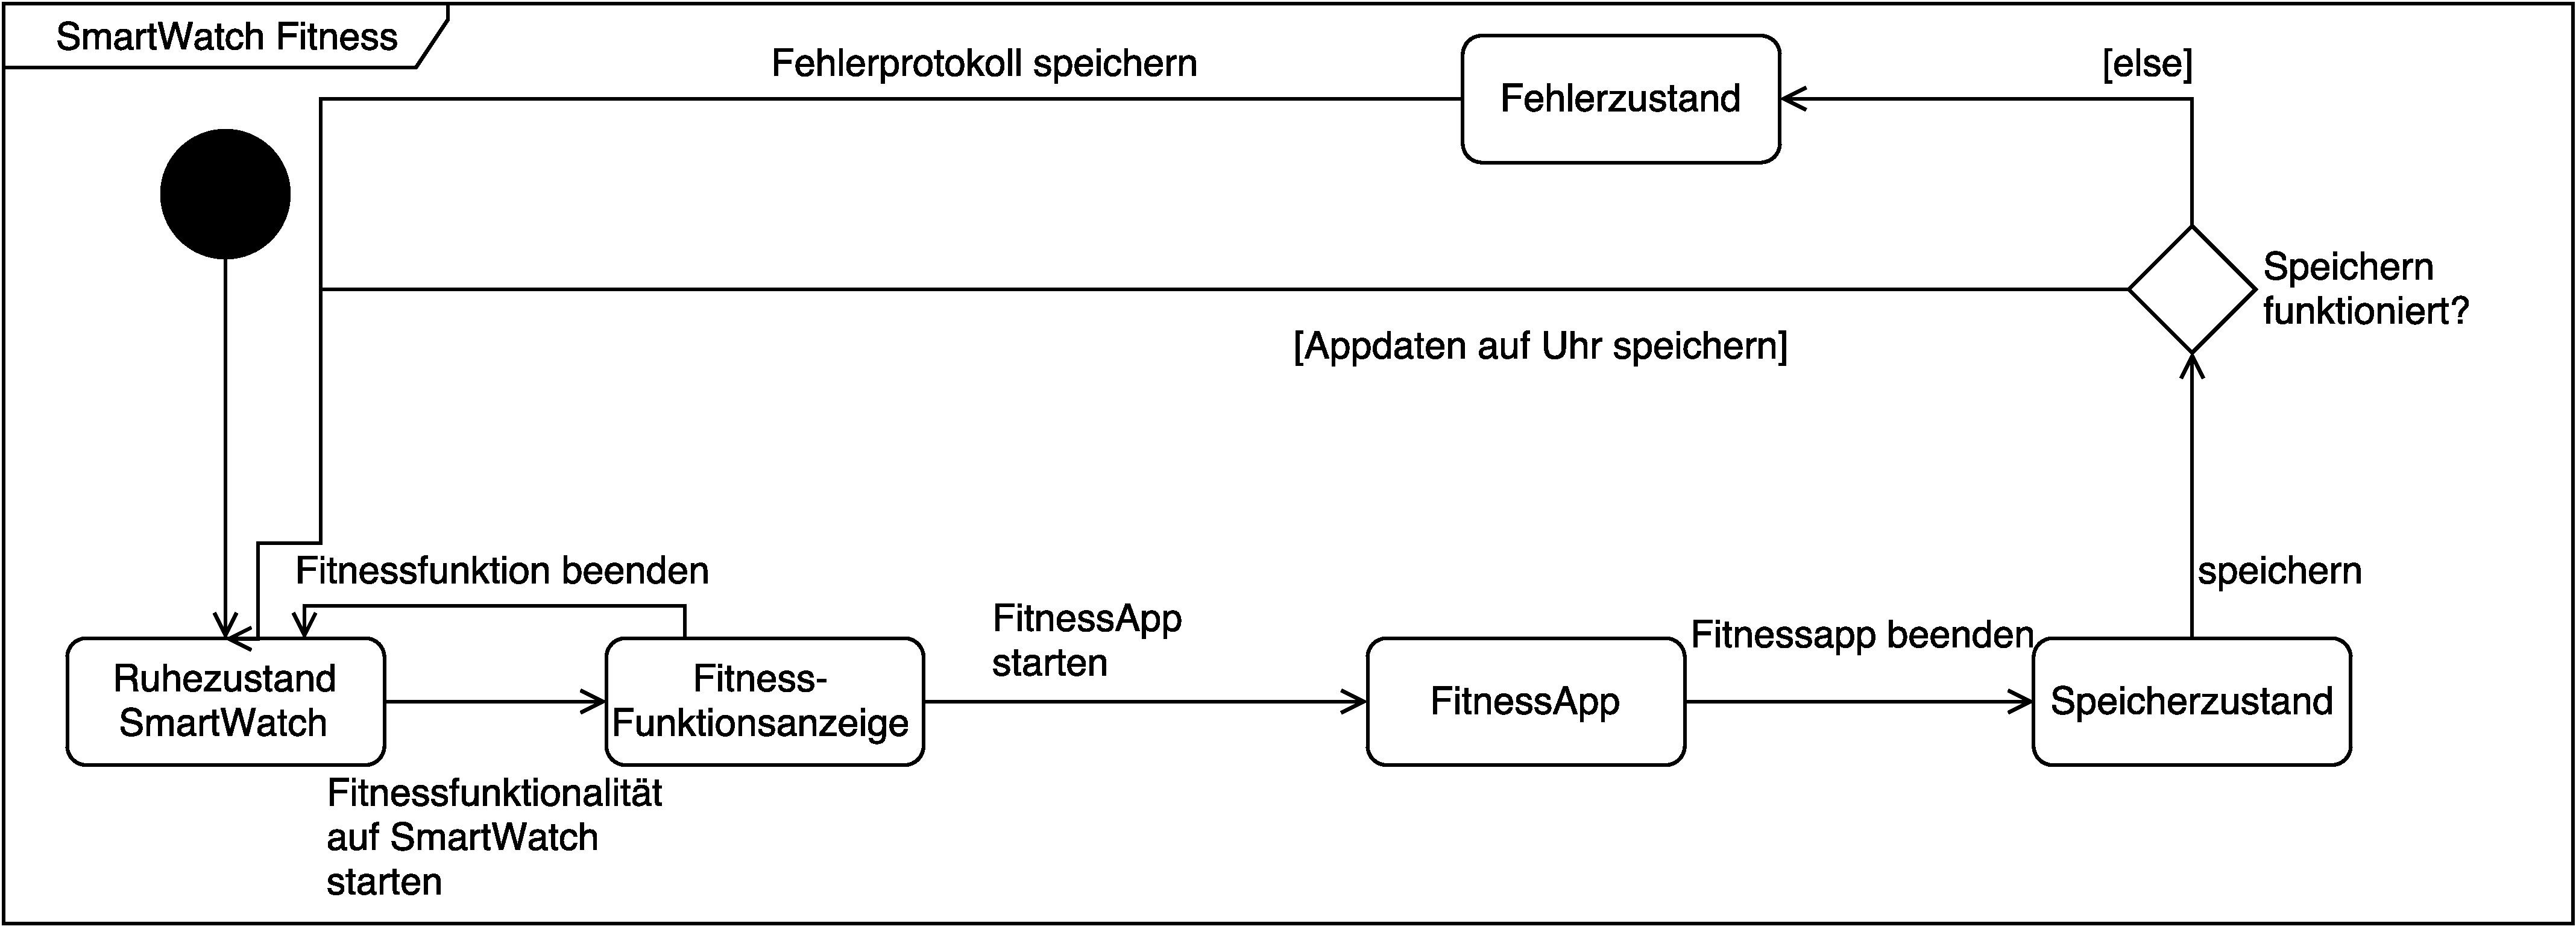
\includegraphics[width=\textwidth]{img/stateFitness}
\caption[State Diagram: Fitness]{Verhalten der SmartWatch beim starten der Fitnessapp.}
\label{fig:stateFitness}
\end{figure}
Wenn die \textit{native Fitnessfunktionalität} der \textit{SmartWatch} benutzt werden will, muss die Uhr zunächst aus dem Ruhezustand geholt werden. Anschließend wird über das Menü die \textit{Fitnessapp} ausgewählt und bestätigt. Anschließend wird die Routine zur Aktivitätsaufzeichnung ausgeführt. Sobald diese beendet ist, versucht die \textit{SmartWatch} die Fitnessdaten im \textit{internen Speicher} abzulegen. Vorausgesetzt der \textit{Speichervorgang} war erfolgreich, werden die Daten auf dem internen Speicher abgelegt. Bei einem Fehler während des Speicherns, werden die Daten gelöscht und ein Fehlerprotokoll erstellt Abb. \ref{fig:stateFitness}.\\
\begin{figure}[h]
\centering\
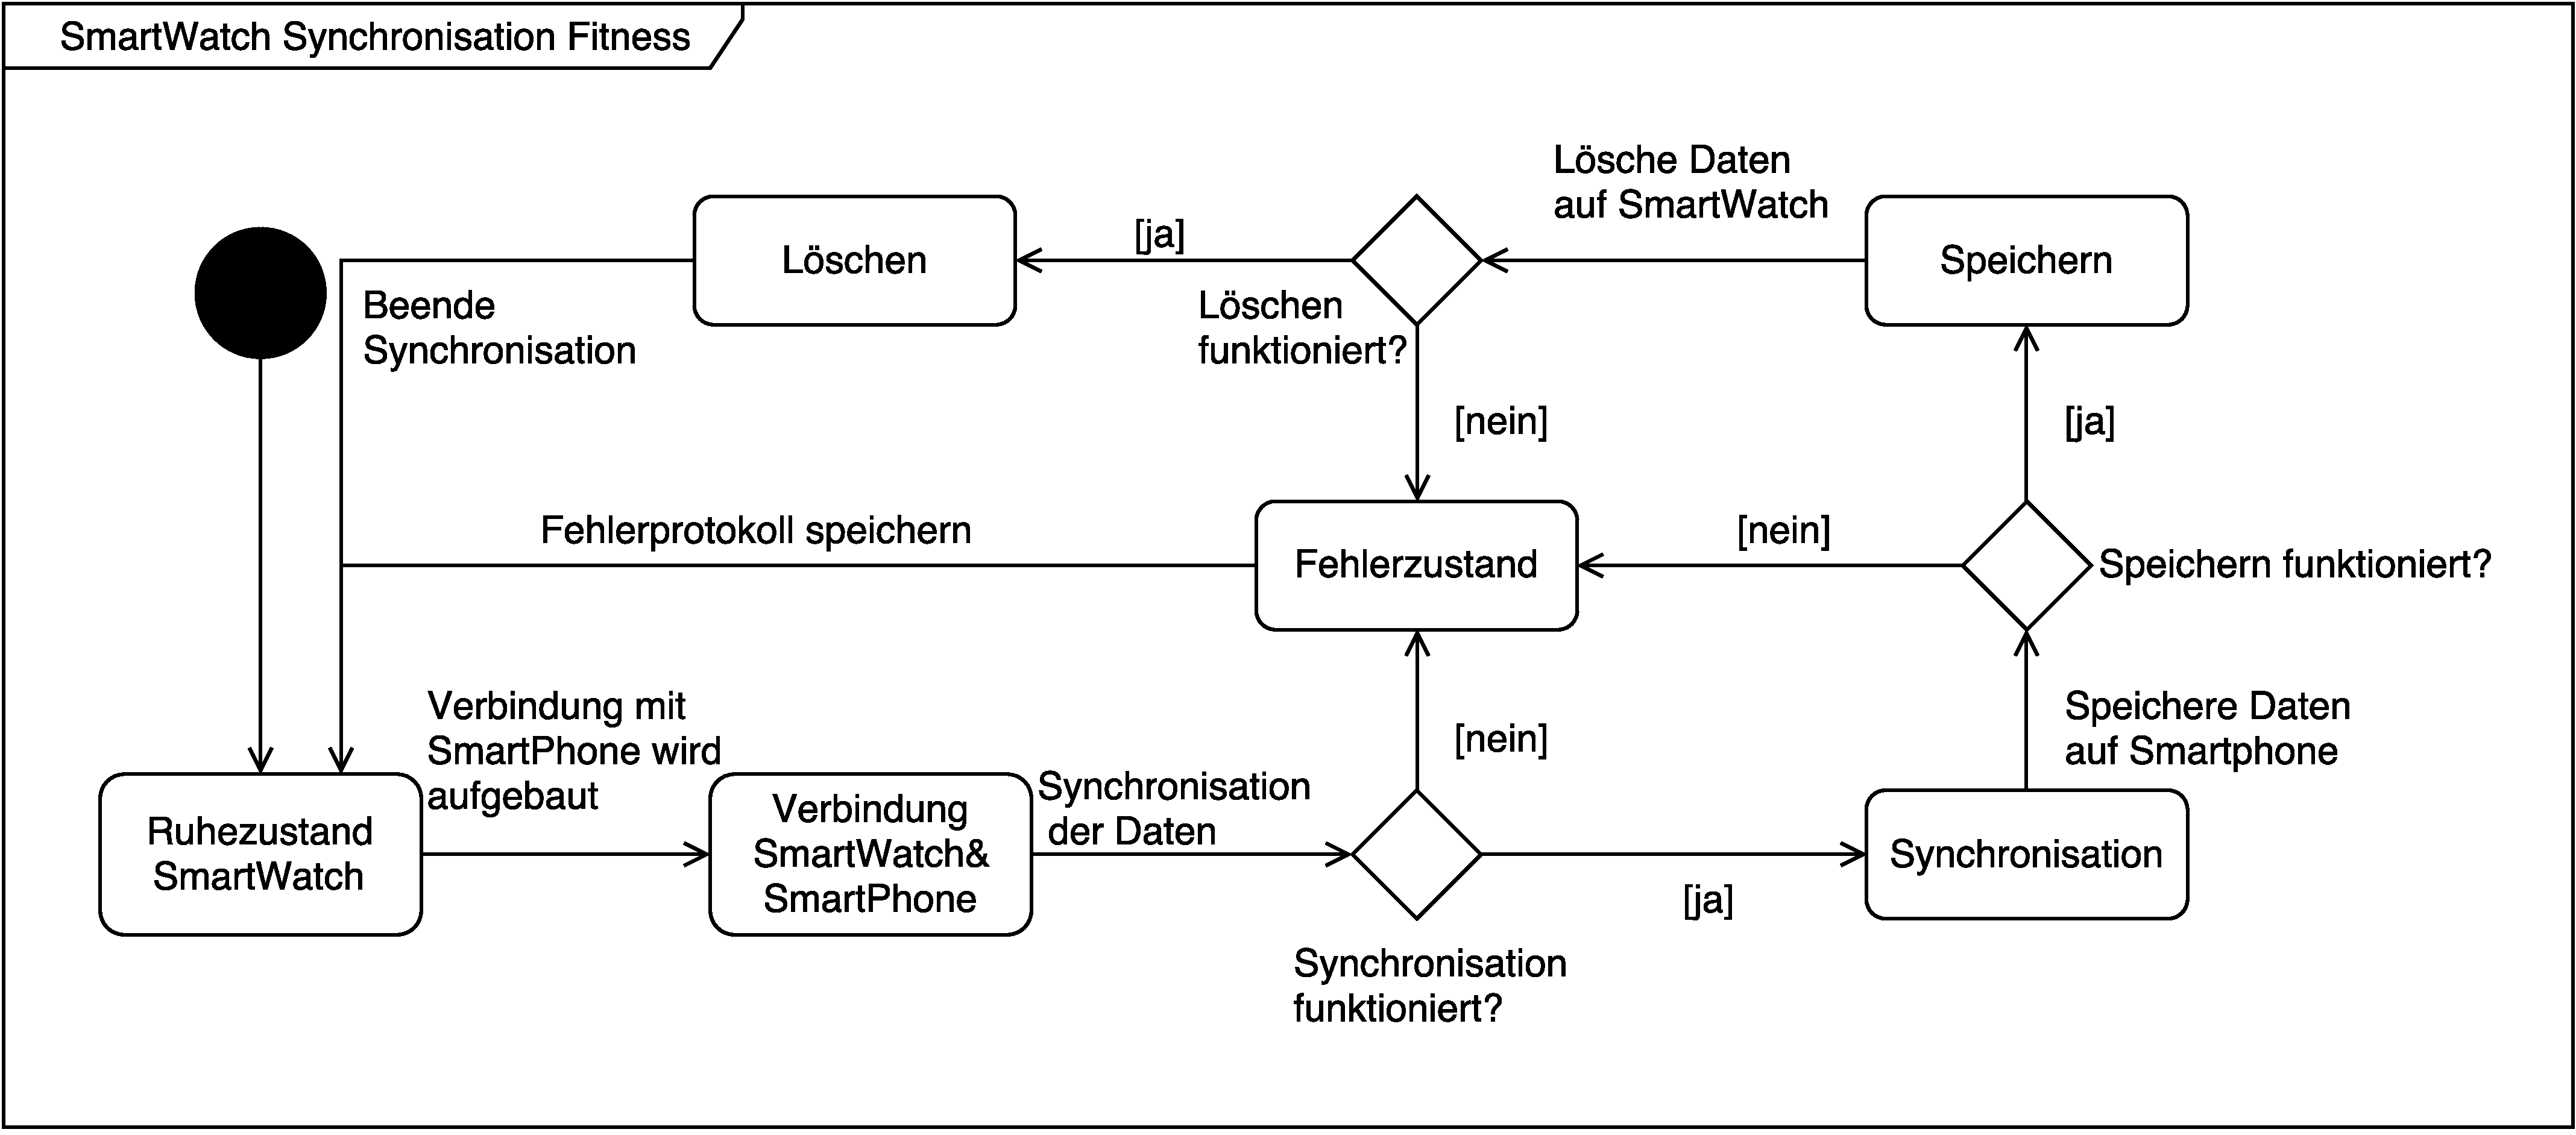
\includegraphics[width=\textwidth]{img/stateSync}
\caption[State Diagram: Synchronisation]{Verhalten der SmartWatch beim Synchronisieren der Fitnessaktivitäten mit dem SmartPhone.}
\label{fig:stateSync}
\end{figure}
Nachdem eine \textit{Fitnessaktivität} beendet wurde und die \textit{Fitnessdaten} auf der \textit{SmartWatch} zwischengelagert wurden, wird versucht bei der nächsten Verbindung mit dem \textit{SmartPhone}, die \textit{Daten} von der \textit{Uhr} auf das \textit{SmartPhone} zu übertragen Abb. \ref{fig:stateSync}. Voraussetzung dafür ist eine erfolgreiche \textit{Verbindung} zwischen den beiden Geräten. Sobald die \textit{Verbindung} steht, wird mit dem \textit{Synchronisationsvorgang} begonnen. Bei diesem werden zunächst die \textit{Daten} von der \textit{Uhr} auf das \textit{Telefon} gespeichert, um einen möglichen Datenverlust zu vermeiden. Anschließend werden die \textit{Daten} von der \textit{SmartWatch} gelöscht und die \textit{Synchronisation} beendet. Sollte im Verlauf der \textit{Synchronisation} ein Fehler auftreten, wird die \textit{Synchronisation} abgebrochen und ein \textit{Fehlerprotokoll} erstellt. \\
\begin{figure}[h]
\centering\
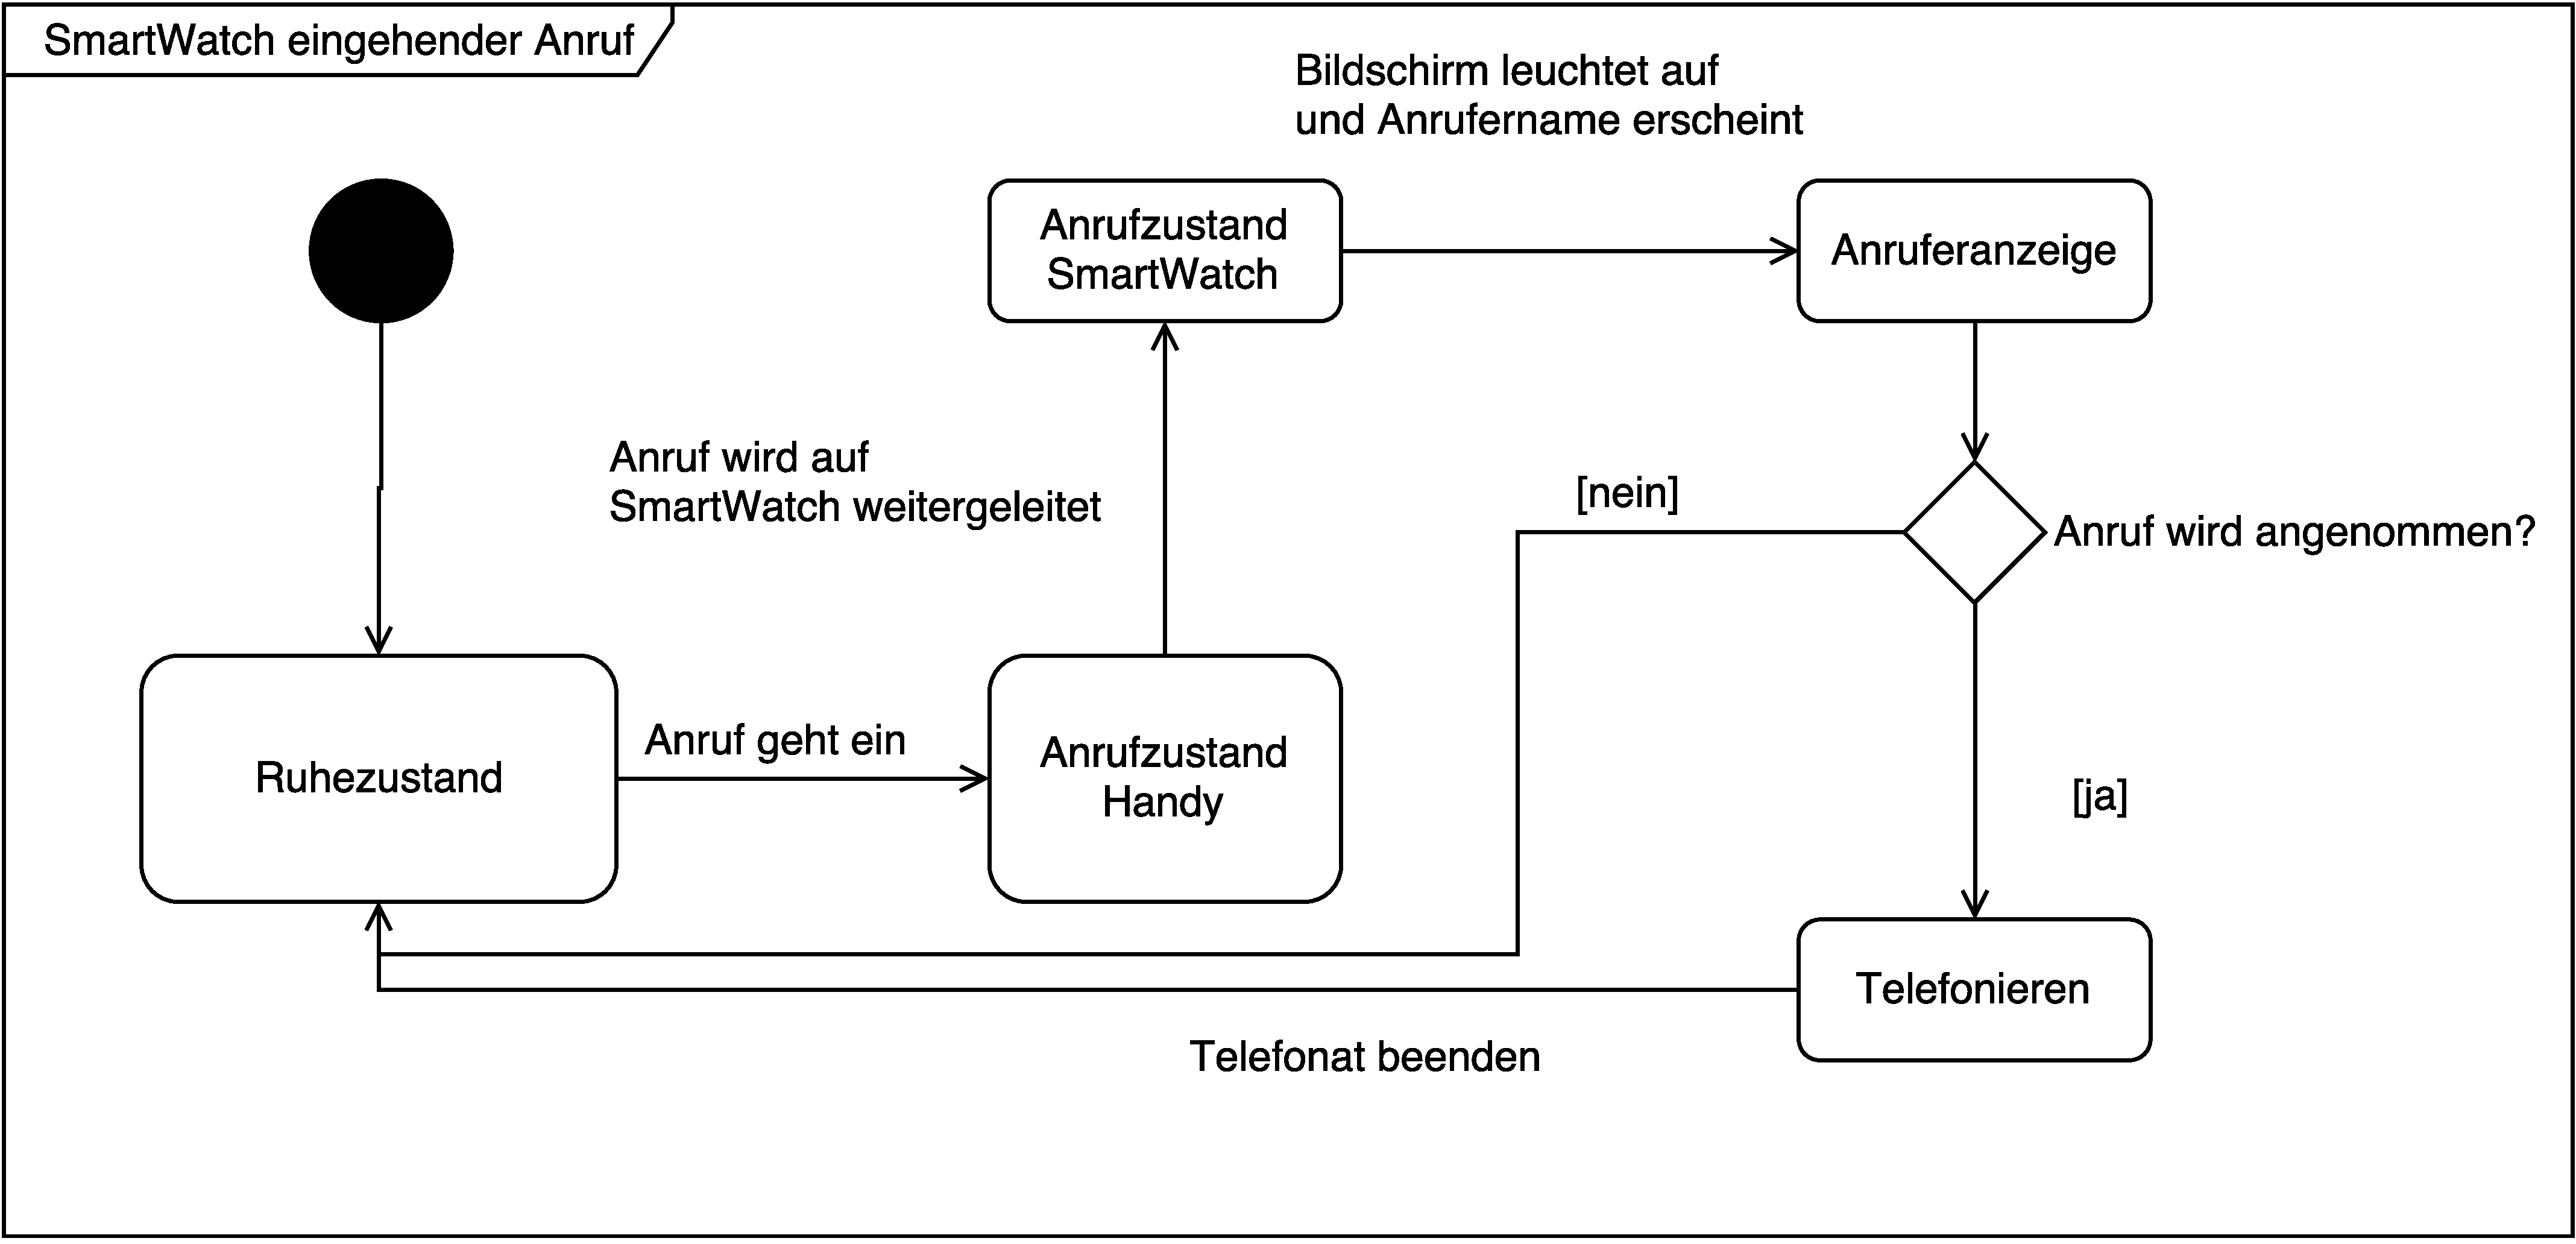
\includegraphics[width=\textwidth]{img/stateAnrufEingehend}
\caption[State Diagram: eingehender Anruf]{Verhalten der SmartWatch bei einen eingehenden Anruf.}
\label{fig:stateAnrufEingehend}
\end{figure}
Als nächstes wird das Verhalten der \textit{SmartWatch} bei einem \textit{eingehenden Anrufen} näher betrachtetAbb. \ref{fig:stateAnrufEingehend}. Zunächst befinden sich sowohl \textit{Handy} als auch \textit{Uhr} im \textit{Ruhezustand}. Sobald ein \textit{Anruf} eingeht, wechselt zuerst das \textit{SmartPhone} in den \textit{Anrufzustand} und gibt ein Signal an die \textit{Uhr} weiter. Sobald die \textit{Uhr} das Signal empfängt, wechselt auch sie in einen \textit{Anrufzustand}. In diesem Zustand, wird die Bildschirmbeleuchtung aktiviert und die \textit{Anruferanzeige} eingeblendet. Diese \textit{Anzeige} ermöglicht es dem Benutzer zu wählen ob er den Anruf entgegen nehmen will oder nicht. Sollte er den Anruf annehmen, wechselt die \textit{SmartWatch} in den Zustand \textit{Telefonieren} und aktiviert die das interne \textit{Mikrophon}. Sobald der Anruf beendet wurde, kehren \textit{Telefon} und \textit{Uhr} in den \textit{Ruhezustand} zurück. \\
\begin{figure}[h]
\centering\
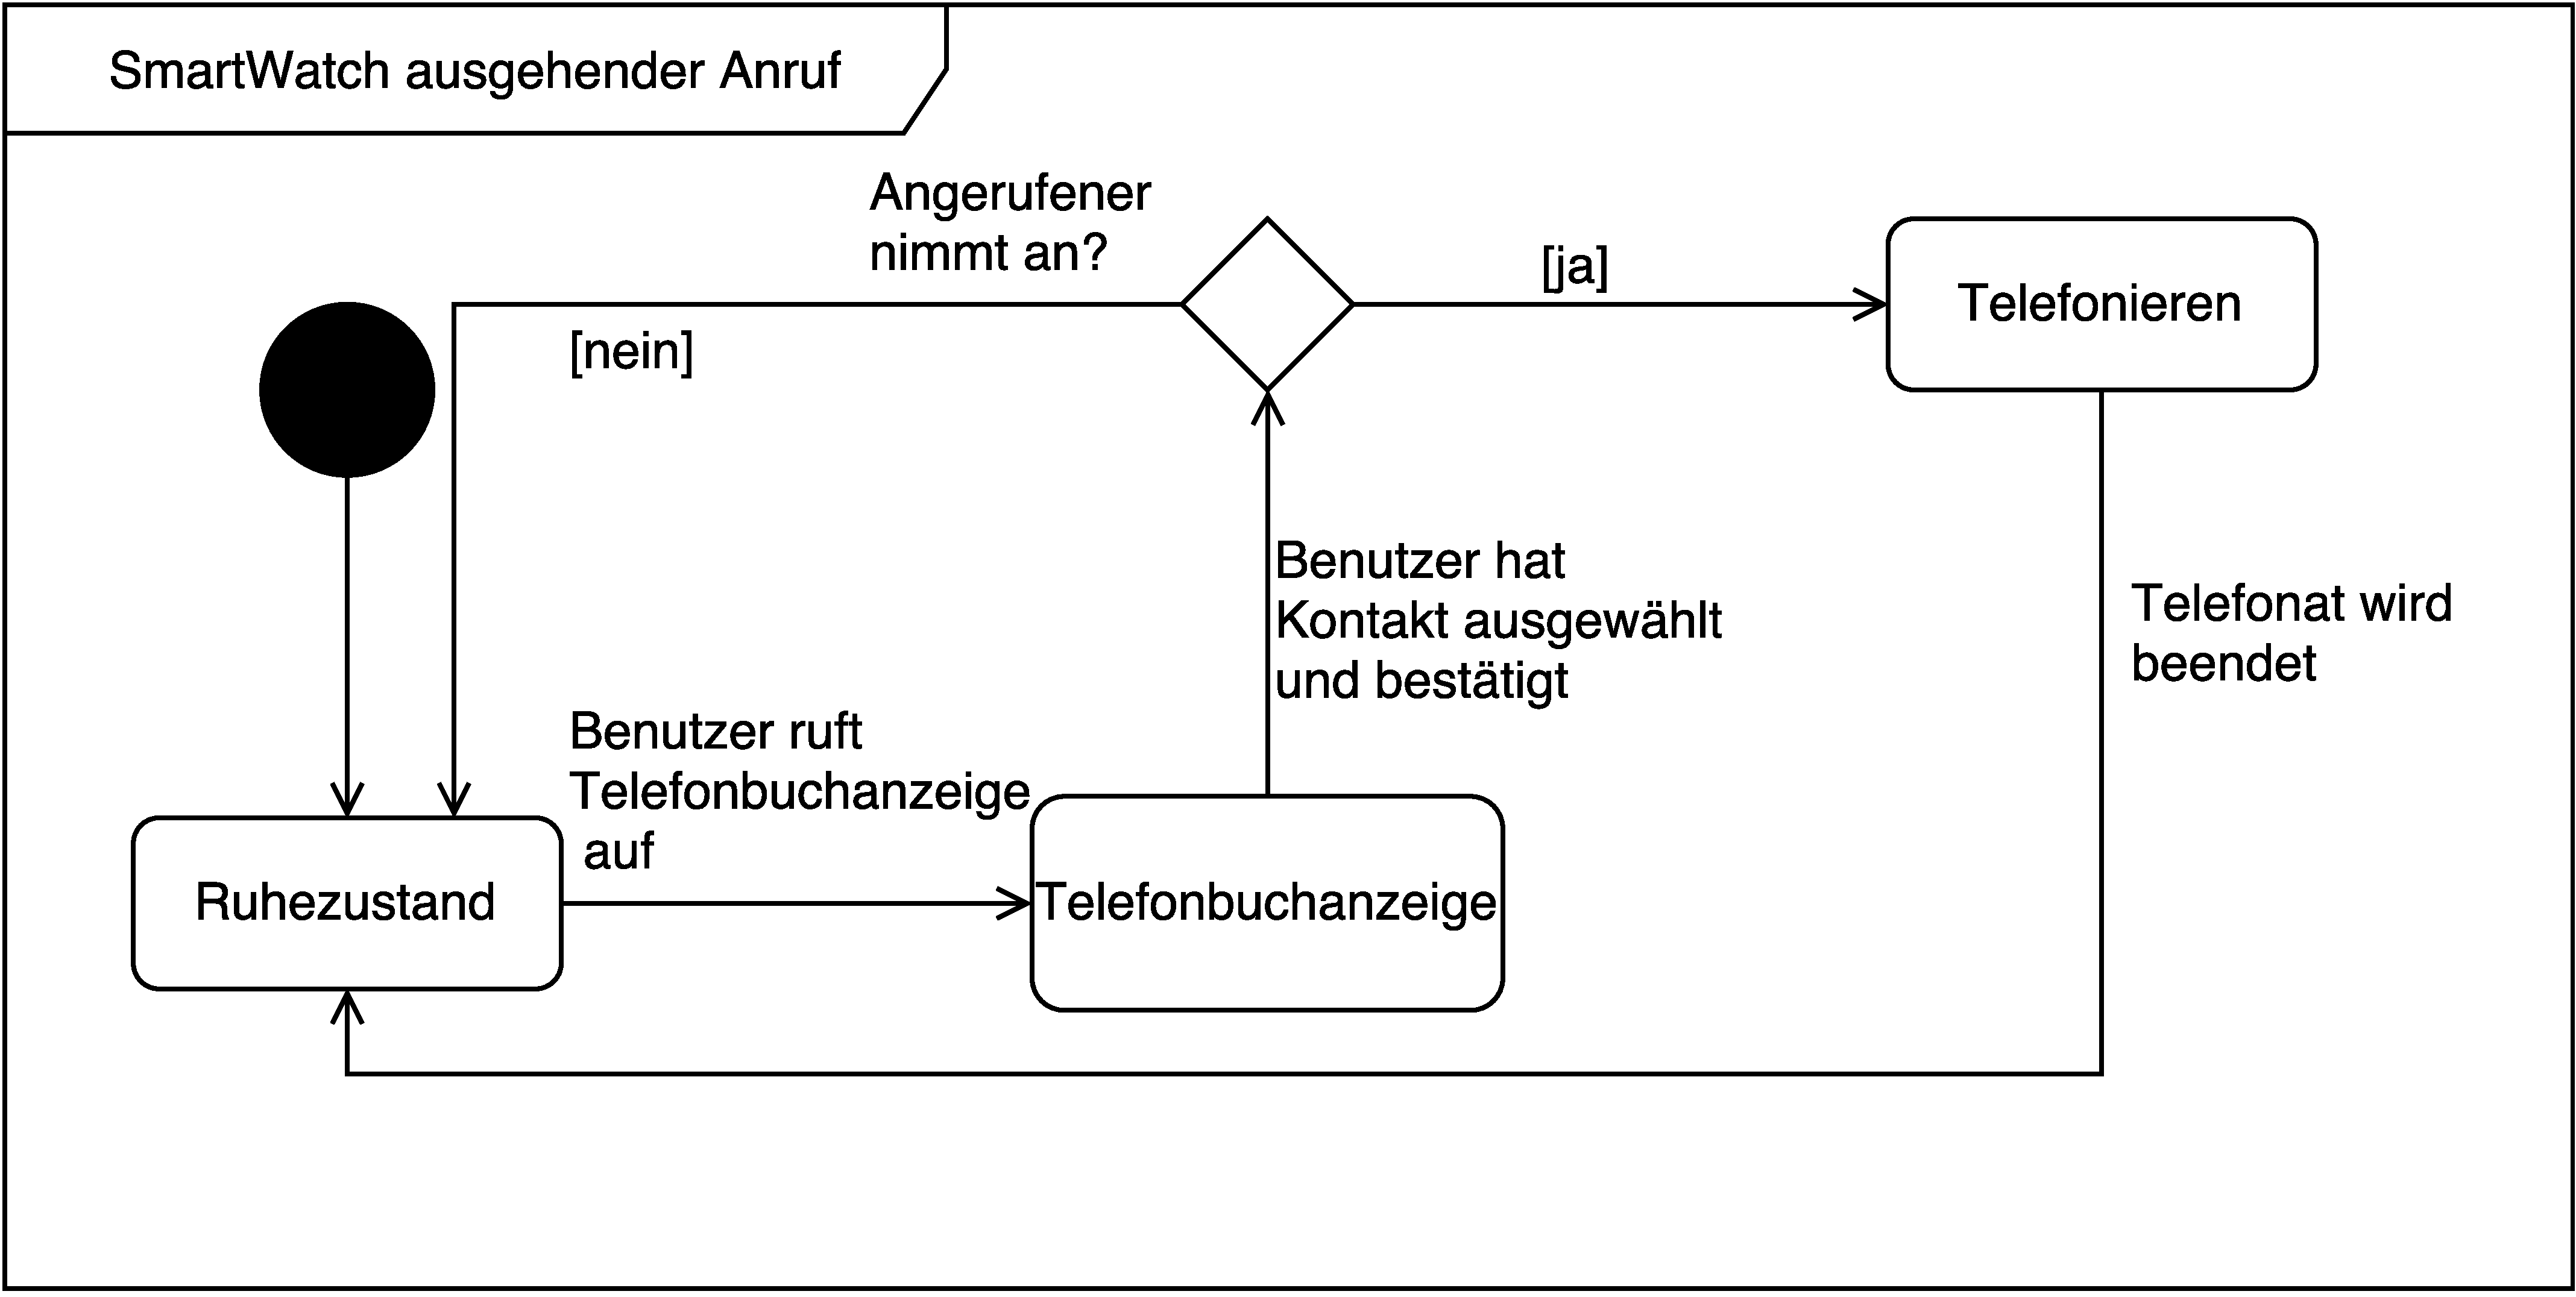
\includegraphics[width=\textwidth]{img/stateAnrufAusgehend}
\caption[State Diagram: ausgehender Anruf]{Verhalten der SmartWatch beim Tätigen eines Anrufs.}
\label{fig:stateAnrufAusgehend}
\end{figure}
Die von uns entwickelte \textit{SmartWatch} soll nicht nur in der Lage sein, Anrufe anzunehmen sondern auch fähig sein \textit{Anrufe zu tätigen} Abb. \ref{fig:stateAnrufAusgehend}. Auch hier wird wieder davon ausgegangen, dass sich beide Geräte im \textit{Ruhezustand} befinden. Beendet wird dieser durch das Aufrufen der \textit{Telefonbuchanzeige} auf der \textit{SmartWatch}. Sobald der Benutzer einen Kontakt über die \textit{SmartWatch}aus dem Telefonbuch des \textit{SmartPhones} gewählt hat, wird die \textit{Anruffunktionalität} eingeleitet. Sollte der Angerufene das Telefonat annehmen wird auch hier in den Zustand \textit{Telefonieren} gewechselt. Dieser Zustand verhält sich genauso wie bei einem \textit{eingehenden Anruf}. Nach Beendigung des Gesprächs wechseln beide Geräte wieder in den \textit{Ruhezustand}.

\section{Timing Diagram}
Um zeitliche Abläufe besser zu verdeutlichen, werden die Anforderungen aus den Requirements \textbf{Connection.02} und \textbf{Notification.02} mittels Timing Diagrams modelliert. Durch das Requirement \textbf{Connection.02} wird definiert, dass der Verbindungsaufbau zwischen Smartwatch und Smartphone in maximal 4 Sekunden dauern darf. Das entsprechende Timing Diagram ist in Abbildung~\ref{fig:timing_diagram_pairing} abgebildet. Dieses Diagramm enthält auch das in Phase 3 hinzugefügte \textit{Satisfy-Callout} um die Abhängigkeit mit Requirement \textbf{Connection.02} besser zu verdeutlichen.

\begin{figure}
\centering\
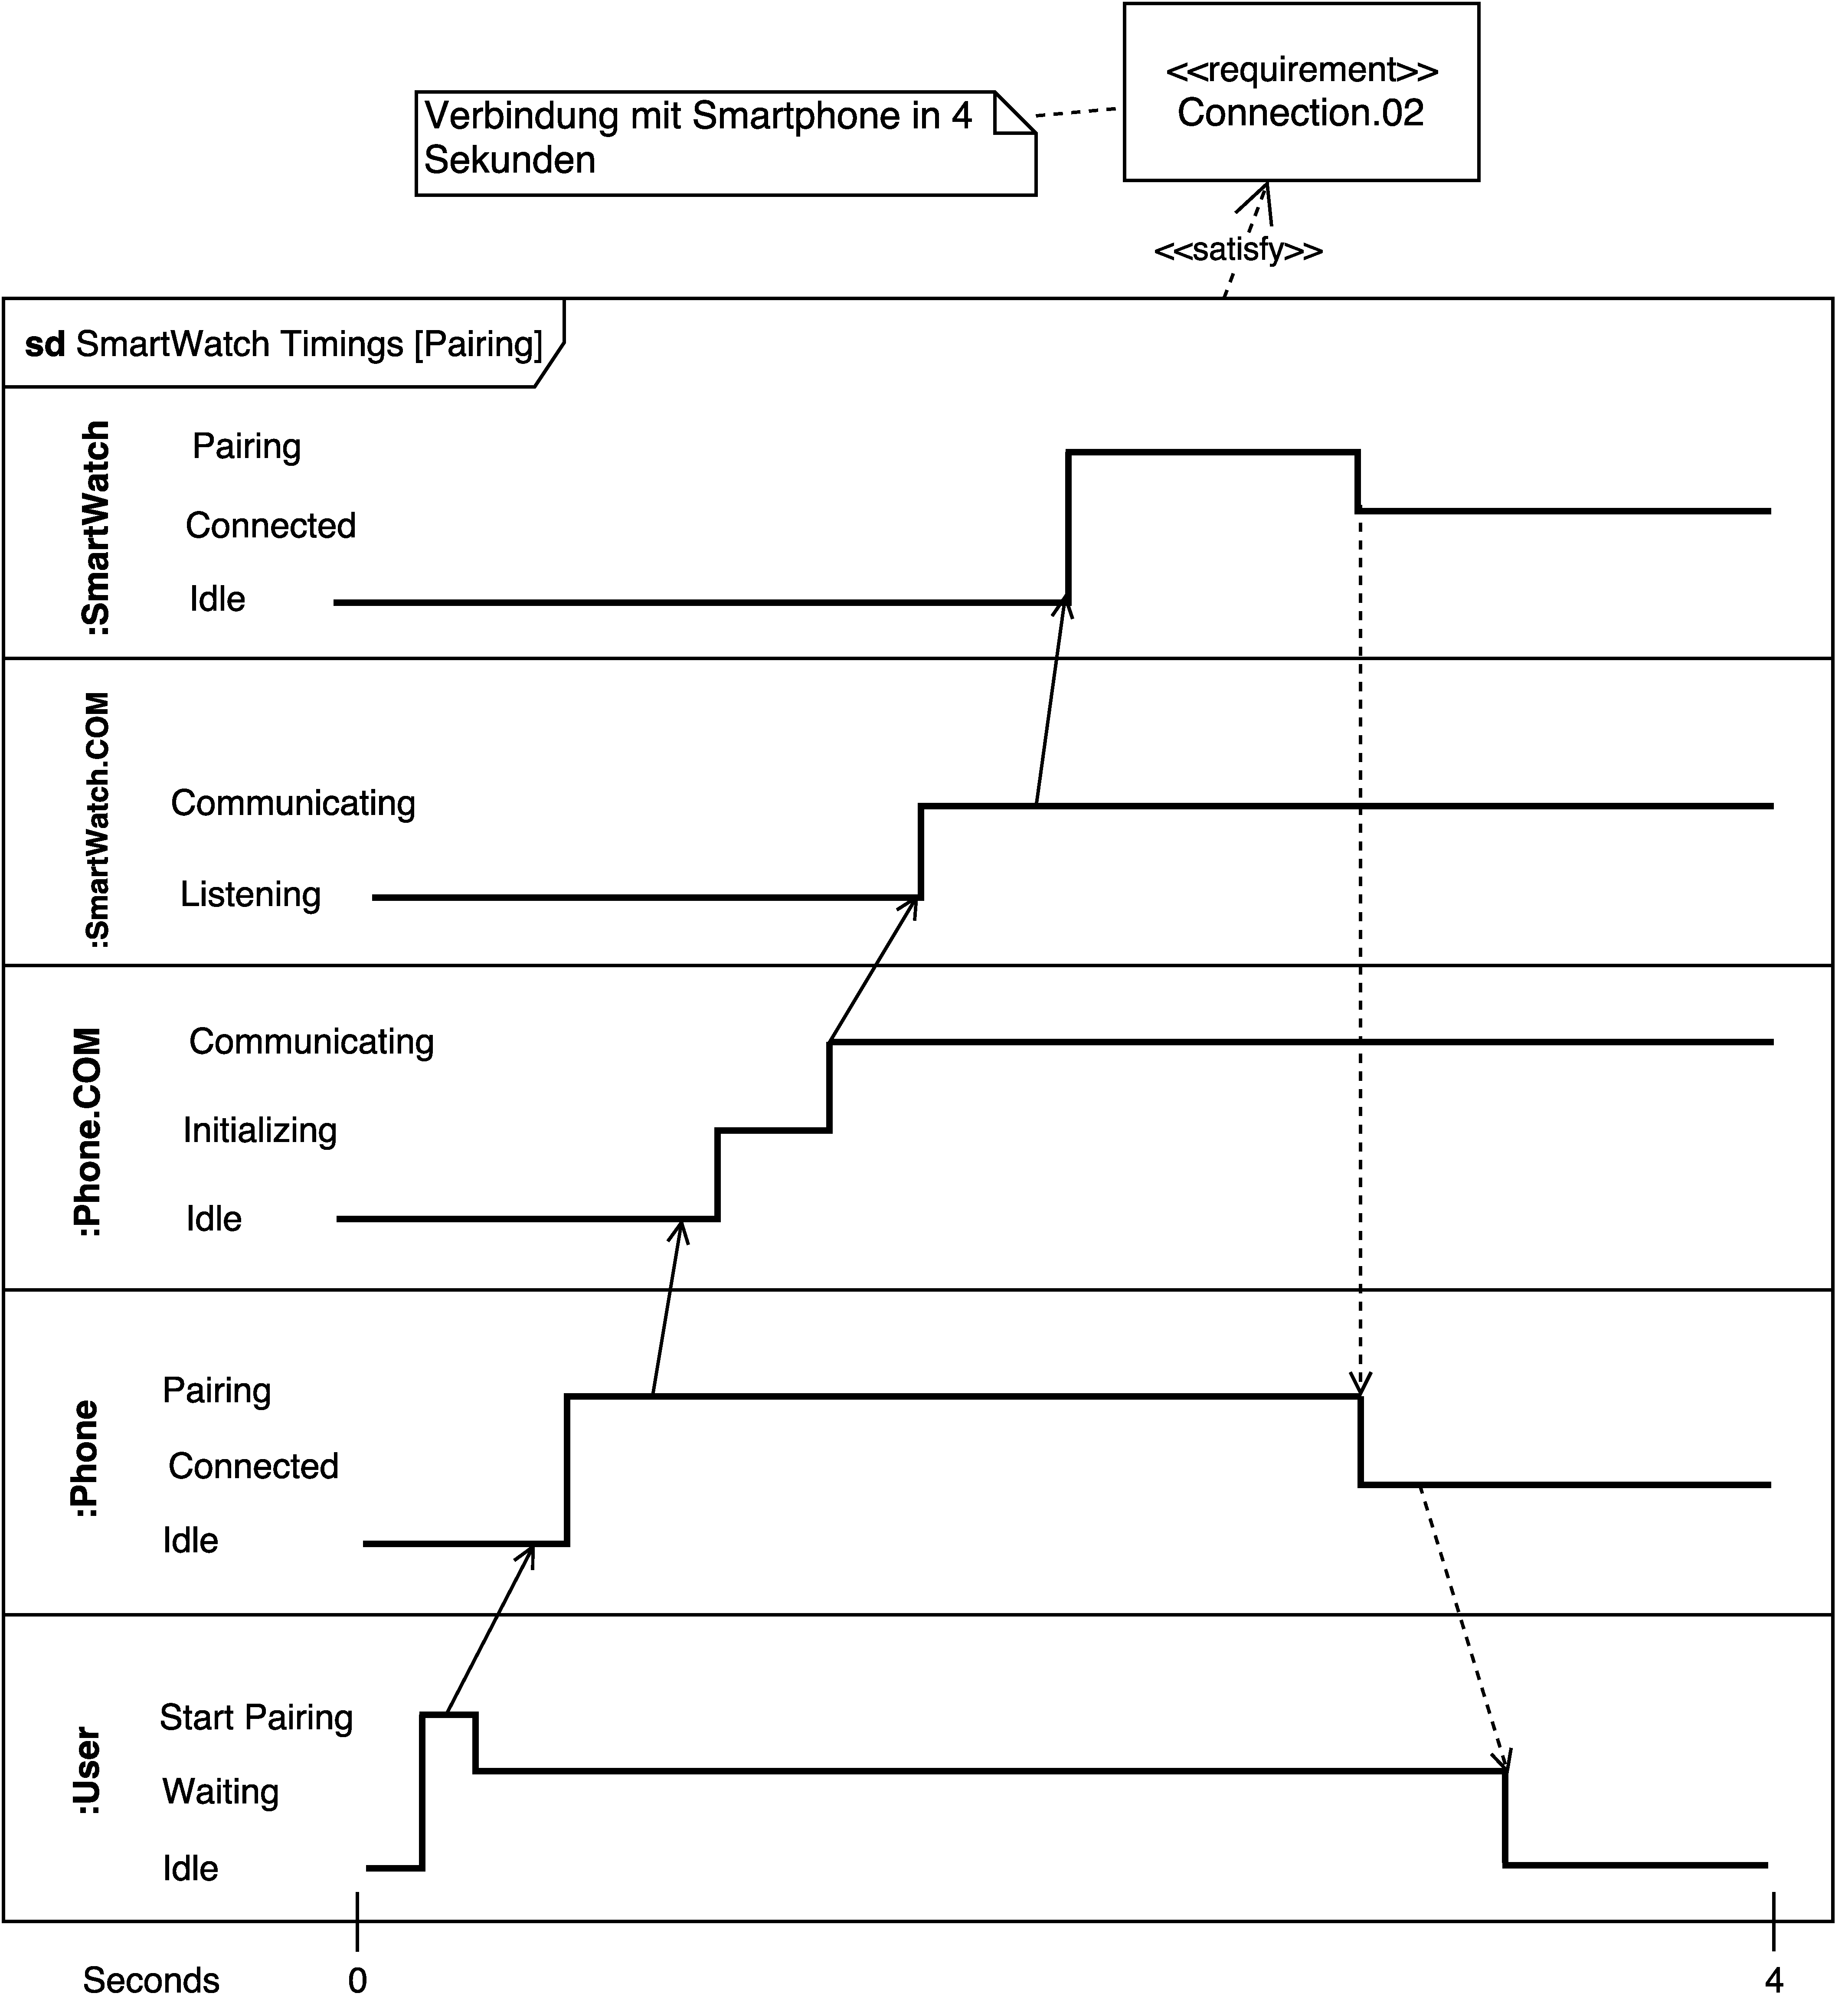
\includegraphics[width=12cm]{img/timing_diagram_pairing}
\caption[Timing Diagram: Pairing]{Modellierung der Anforderungen aus Requierement \textbf{Connection.02} als Timing Diagram. }
\label{fig:timing_diagram_pairing}
\end{figure}

Die Zeit bis zum Anzeigen einer \gls{Notification} wird im Requirement \textbf{Notification.02} detailliert beschrieben. Aus dem Requirement folgt, dass \glspl{Notification} innerhalb einer Sekunde auf der Smartwatch angezeigt werden müssen. Dieses Verhalten ist in Abbildung~\ref{fig:timing_diagram_notifications} dargestellt.

\begin{figure}
\centering\
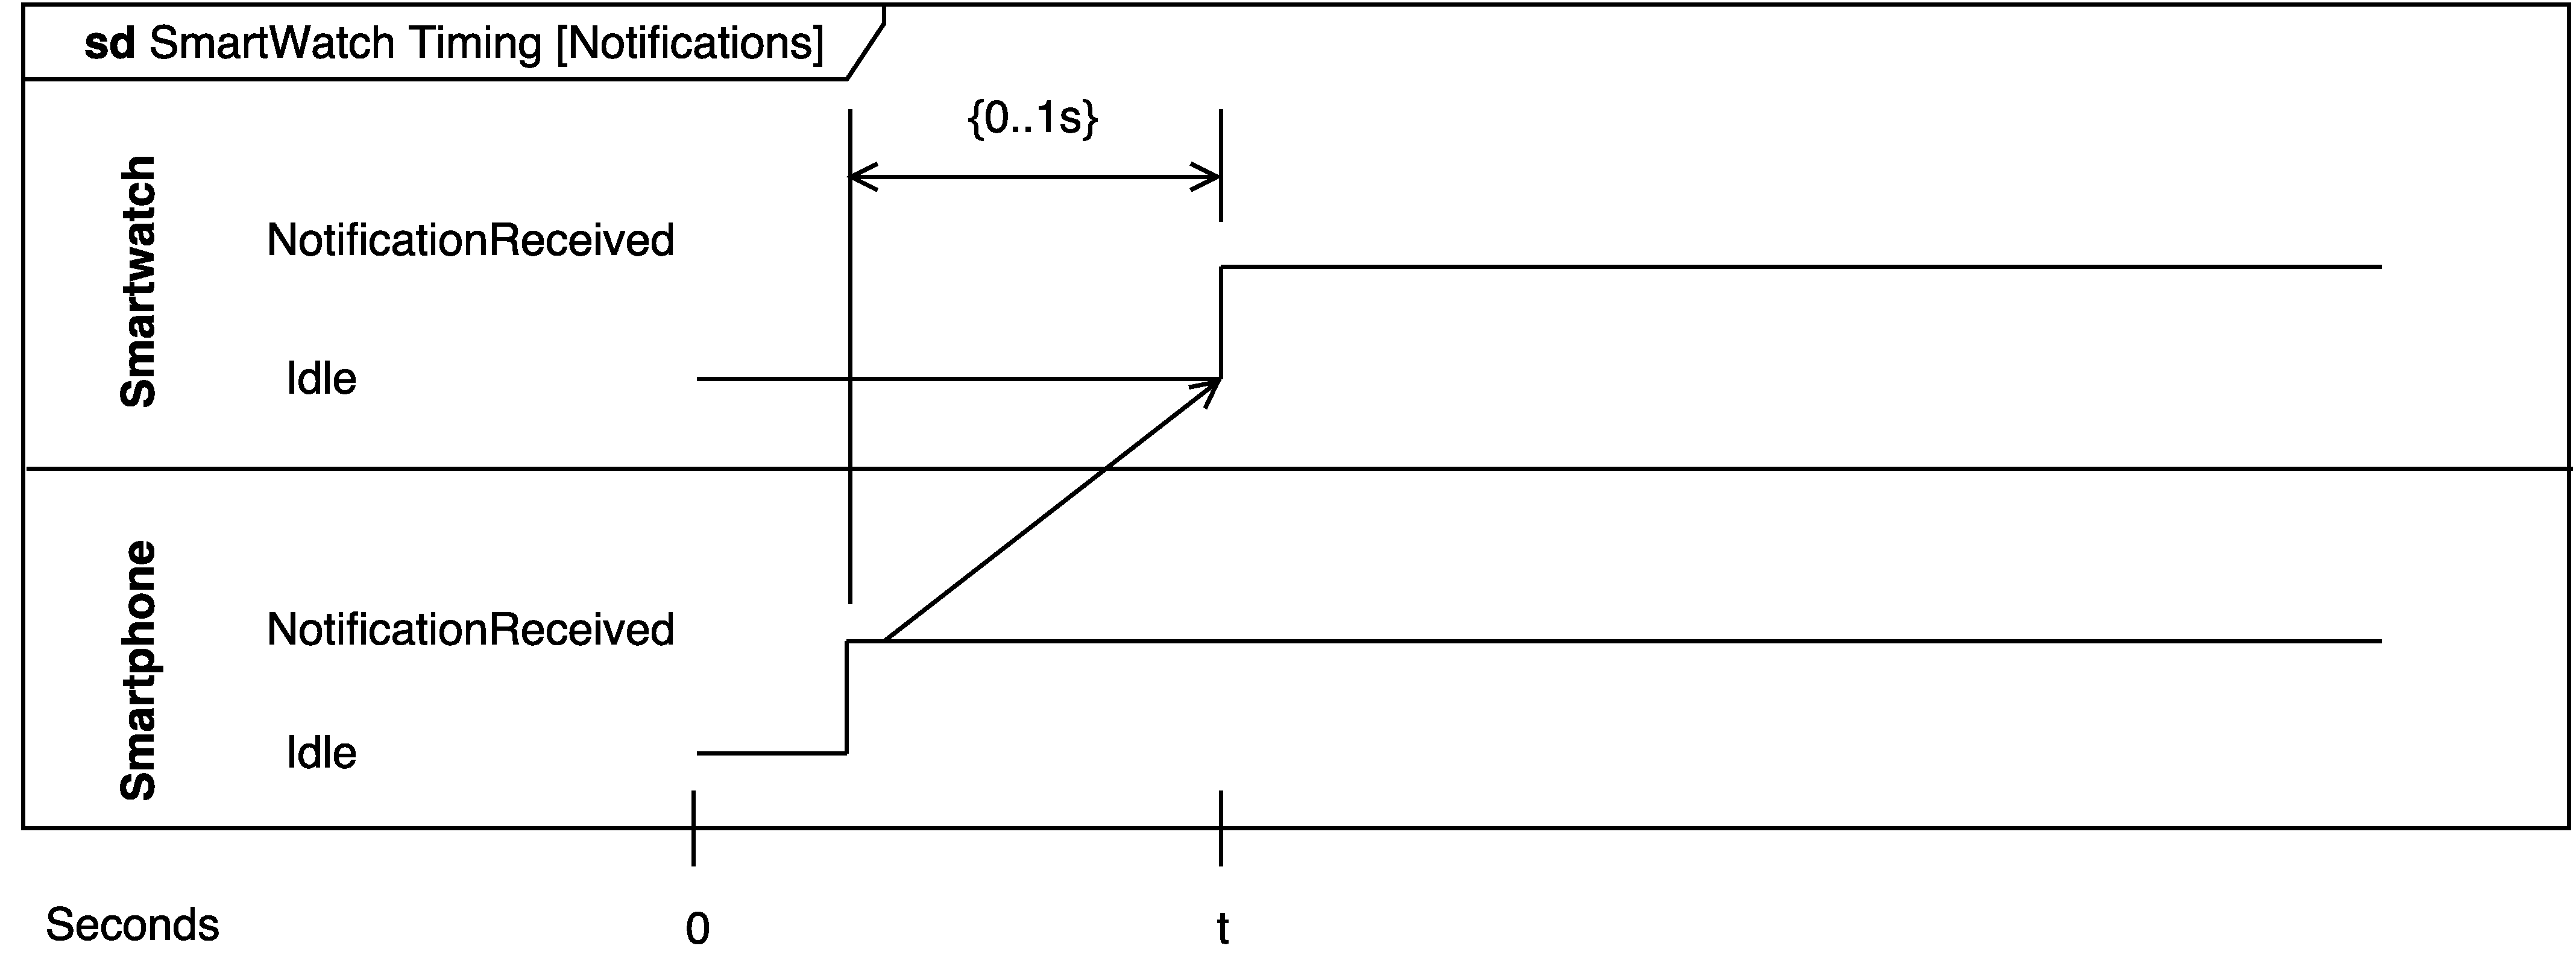
\includegraphics[width=14cm]{img/timing_diagram_notifications}
\caption[Timing Diagram: Notifications]{Modellierung der Anforderungen aus Requirement \textbf{Notification.02} bezüglich der Anzeige von \glspl{Notification} als Timing Diagram.}
\label{fig:timing_diagram_pairing}
\end{figure}

